% 第1章 绪论
\chapter{绪论}

\leavevmode\usetikzlibrary{arrows.meta, positioning, calc, decorations.pathmorphing, shapes.geometric}

固体力学的核心任务之一，是描述材料从连续变形到最终破坏的全过程。断裂与损伤是工程结构失效的最常见形式，然而经典连续介质力学在处理这类强不连续问题时遭遇了深层次的困难。本章首先回顾经典连续介质力学的基本假设及其在断裂问题中的根本局限（1.1节），进而追溯非局部理论的发展脉络（1.2节），引出近场动力学的诞生（1.3节），阐明其核心思想与基本特征（1.4节），并按研究方向系统梳理其发展历程与研究现状（1.5节），最后介绍本书的结构与阅读建议（1.6节）。本章的目的不在于给出严格的数学推导，而在于回答两个基本问题：为什么需要近场动力学，以及近场动力学是什么。严格的数学框架将在第2章建立，近场动力学与经典连续介质力学的关系将在第3章详细分析。

\section{经典连续介质力学的局限与挑战}

经典连续介质力学（classical continuum mechanics，简称 CCM）自 18 世纪以来一直是固体力学与工程分析的基石。它以两个基本假设为前提。一是连续性假设，认为材料占据的空间区域可以逐点定义密度、位移、应力等场量。二是局部作用假设，认为材料点只与其无穷小邻域内的物质发生相互作用，其力学状态完全由该点处的变形梯度决定。在这两个假设之下，线动量平衡可以写成含空间导数的偏微分方程
\[
  \nabla\cdot\boldsymbol{\sigma}+\mathbf{b}=\rho\ddot{\mathbf{u}}
\]
其中 $\boldsymbol{\sigma}$ 为 Cauchy 应力张量，$\mathbf{b}$ 为体力密度，$\mathbf{u}$ 为位移场，$\rho$ 为质量密度。应力与应变通过本构方程相联系，工程问题大多借助有限元等数值方法求解这一局部微分方程系统。这套框架在结构分析中取得了巨大成功，但它的两个基本假设恰恰构成其处理断裂问题时困境的根源 \cite{Silling2000}。

第一个困难来自位移场的不连续。断裂的本质是在材料中形成位移不连续面，即裂纹面。在不连续面上，位移对空间坐标的偏导数没有定义，而经典理论恰恰用这些偏导数来表示相邻材料点之间的相对位移与相互作用力。正如 Silling 所指出的 \cite{Silling2000}，固体力学中诸多基本问题恰恰以这种自发形成的不连续为核心，而连续介质力学的数学框架在某种程度上并不适合描述这类问题，因为沿不连续处所需的空间偏导数按定义不存在。传统的处理方式是把裂纹作为额外的人为对象引入：预先假定裂纹位置，将其表面设为自由边界，再附加专门的断裂准则决定其扩展。这种先假设、再验证的范式在裂纹路径未知、多裂纹相互作用或裂纹分叉的情形下变得极为困难。

第二个困难是裂纹尖端场的奇异性。对线弹性材料中的平面裂纹，Irwin 的分析表明 \cite{Irwin1957}，裂纹尖端附近的应力场具有
\[
  \sigma_{ij}\sim\frac{K_I}{\sqrt{2\pi r}}\qquad(r\to 0)
\]
的形式，其中 $K_I$ 为 I 型应力强度因子，$r$ 为距裂尖的距离。当 $r$ 趋于零时，应力趋于无穷大，这在物理上不可接受。这一奇异性意味着经典弹性理论无法给出裂尖处的真实应力状态，必须借助应力强度因子或能量释放率等概念加以回避。Griffith 最早从能量角度建立了断裂准则 \cite{Griffith1921}，认为当裂纹扩展所释放的弹性能足以支付新表面所需的表面能时，裂纹发生失稳扩展。该准则给出的临界应力为
\[
  \sigma_c=\sqrt{\frac{2E\gamma}{\pi a}}
\]
其中 $E$ 为弹性模量，$\gamma$ 为表面能密度，$a$ 为裂纹半长。这一公式同时暴露出 Griffith 准则的根本局限。当裂纹尺寸 $a$ 趋于零时，临界应力趋于无穷大，因此该准则无法回答无初始裂纹的完整构件在多大载荷下萌生裂纹这一基本问题。此外，它只能判定裂纹在什么条件下扩展，既不能预测扩展方向，也不能处理裂纹分叉、跳跃以及多裂纹之间的相互作用。Irwin 的应力强度因子方法 \cite{Irwin1957} 在工程上十分有效，但同样需要预知裂纹的几何与位置，本质上属于裂纹扩展准则而非裂纹萌生理论。裂纹尖端应力场的形式如图\ref{fig:crack-singularity}所示：当距裂纹尖端距离 $r \to 0$ 时，应力按 $r^{-1/2}$ 发散，这正是经典弹性理论预测的应力奇异性——裂纹尖端应力趋于无穷，在物理上并不合理。

\begin{figure}[htbp]
  \centering
  \begin{tikzpicture}[scale=0.9]
    % 左：含裂纹平板
    \draw[thick] (-3,1.5) rectangle (3,-1.5);
    \draw[ultra thick] (-1.5,0) -- (1.5,0);
    \draw[-Stealth, thick] (-2,2) -- (-2,1.5);
    \draw[-Stealth, thick] (2,2) -- (2,1.5);
    \draw[-Stealth, thick] (-2,-2) -- (-2,-1.5);
    \draw[-Stealth, thick] (2,-2) -- (2,-1.5);
    \node at (-2,2.3) {$\sigma$};
    \node at (2,2.3) {$\sigma$};
    \node[below] at (0,-1.8) {(a) 含裂纹平板};
    % 右：σ-r曲线
    \begin{scope}[xshift=6cm]
      \draw[-Stealth] (0,0) -- (3.5,0) node[right] {$r$};
      \draw[-Stealth] (0,-1.5) -- (0,2.5) node[above] {$\sigma$};
      \draw[dashed] (0,0) -- (0,2.2);
      \draw[thick, blue, domain=0.3:3, samples=50] plot (\x, {1.2/sqrt(\x)});
      \node[blue, right] at (1.5,1.0) {$\sigma \sim r^{-1/2}$};
      \node[red, left] at (0,2.0) {$\infty$};
      \node[below] at (1.5,-1.8) {(b) 裂尖应力奇异性};
    \end{scope}
  \end{tikzpicture}
  \caption{裂纹尖端应力奇异性示意，经典弹性理论预测裂尖处应力趋于无穷大}
  \label{fig:crack-singularity}
\end{figure}

第三个困难来自材料软化导致的数学不适定与网格依赖。1958 年，Kachanov 以连续损伤力学开创了对材料劣化的连续描述 \cite{Kachanov1958}，通过损伤变量刻画刚度的退化。然而当损伤本构包含应变软化段时，边值问题将失去适定性。Ba\v{z}ant 与 Belytschko 以一维应变软化杆为例给出了精确解 \cite{BazantBelytschko1985}，证明变形局部化在数学上收敛于零测度集合，损伤带的宽度随网格细化而趋于零，能量耗散也随之趋于零，数值结果对网格产生灾难性的依赖。换言之，损伤被数值压缩进零体积，完全损伤区（completely damaged zone，简称 CDZ）失去物理意义，这正是连续损伤力学在断裂预测中屡屡失效的根源。

为恢复适定性，研究者提出了多种正则化手段。Pijaudier-Cabot 与 Ba\v{z}ant 引入非局部损伤模型 \cite{PijaudierCabotBazant1987}，以特征长度加权的积分平均替代点值；Peerlings 等发展梯度增强损伤模型 \cite{Peerlings1996}，在本构中引入应变的高阶梯度；此外还有微极连续体等含独立转动自由度的理论（其历史脉络见 1.2 节 \cite{Cosserat1909}）。这些方法都引入了内部长度尺度，在一定程度上缓解了网格依赖，但它们大多仍然建立在偏微分方程与应力张量的框架之内，在裂纹萌生、分叉与汇合等强不连续问题面前仍然力不从心，且正则化参数的选取缺乏统一的物理依据。

上述分析表明，断裂问题的困难并非某个细节处理不当，而是源于经典理论以微分描述相互作用这一基本架构。要使不连续的产生与演化成为方程的自然结果，需要一种在数学上自洽、在构造上不以连续位移场为前提的理论。这正是近场动力学试图提供的。图\ref{fig:pd-paradigm}对比了经典连续介质力学、离散方法与近场动力学三种范式对材料点相互作用的不同描述方式。

\begin{figure}[htbp]
  \centering
  
\includegraphics[width=0.85\textwidth]{dimola2022_fig1.png}
  \caption{经典连续介质力学、离散方法与近场动力学对材料点相互作用的描述范式示意（图片来源\cite{Dimola2022}）}
  \label{fig:pd-paradigm}
\end{figure}

\section{非局部理论的起源与发展}

非局部思想在力学中由来已久，其源头可以追溯到 19 世纪。1887 年，Voigt 在晶体弹性的研究中引入比经典 Cauchy 理论更丰富的自由度描述 \cite{Voigt1887}。1909 年，Cosserat 兄弟在《可变形体的理论》（Th\'{e}orie des corps d\'{e}formables）中系统建立了微极连续体理论 \cite{Cosserat1909}，赋予材料点独立的转动自由度，使应力张量不再对称，并引入偶应力。这些工作在当时的框架内属于少数派，却为后来的微结构与梯度理论埋下了伏笔。

现代非局部弹性理论的确立以 Kr\"{o}ner 1967 年的工作为标志 \cite{Kroner1967}。Kr\"{o}ner 提出了第一个长程内聚力弹性模型，材料点之间的相互作用不再局限于无穷小邻域，而是延伸到有限距离。此后，Eringen 及其合作者将这一思想发展为系统的理论体系。Eringen 与 Edelen 于 1972 年建立了非局部弹性的公理化框架 \cite{EringenEdelen1972}，同年 Eringen 给出线性非局部弹性理论，并研究了平面波的色散 \cite{Eringen1972}。在该框架中，应力被表述为整个定义域上应变的泛函，典型形式为
\[
  \sigma_{ij}(\mathbf{x})=\int_V \alpha(|\mathbf{x}'-\mathbf{x}|)\,C_{ijkl}\,\varepsilon_{kl}(\mathbf{x}')\,dV'
\]
其中 $\alpha$ 为随距离衰减的衰减函数（attenuation function），即核函数，它刻画了长程相互作用的强度随距离的变化。当核函数退化为 Dirac 函数时，上式回到经典局部本构关系，可见经典理论是非局部理论的一个极限情形。1983 年，Eringen 进一步指出 \cite{Eringen1983}，若将积分核取为某个微分算子的 Green 函数，则上述积分型本构可以等价地写成微分形式，例如
\[
  (1-l^2\nabla^2)\sigma_{ij}=C_{ijkl}\varepsilon_{kl}
\]
其中 $l$ 为材料内禀长度尺度（intrinsic length scale），即刻画微结构对力学行为影响范围的特征长度。经典本构中不含任何长度参数，应力仅取决于当前点的应变；内禀长度的引入使本构关系能够感知有限空间范围内的非局部效应，其值通常与晶格常数、晶粒尺寸等微结构尺度相联系。这一微分形式的非局部理论在纳米力学中获得了广泛应用。

积分核与长度尺度的引入，使非局部理论能够描述经典理论无法刻画的尺度效应。原子晶格的色散关系对波数的依赖，在非局部弹性中通过核函数的 Fourier 变换自然浮现，而经典弹性理论只能描述长波极限行为。非局部理论还在位错芯结构、表面效应与纳米结构力学中得到了应用，其长度尺度 $l$ 通常与材料的微结构特征尺度相当。但核函数的具体形式及其参数缺乏来自底层物理的直接约束，往往需要借助实验或原子模拟加以标定，这成为非局部理论走向定量预测的一个障碍。

另一条平行的路线是梯度理论。Mindlin 于 1964 年建立了含微结构的线弹性理论 \cite{Mindlin1964}，将应变能密度写为应变及其梯度乃至更高阶导数的函数；Aifantis 等则将梯度项引入塑性本构，用于描述应变局域化 \cite{Aifantis1992}。梯度理论可以看作核函数具有特殊形式的非局部理论，其共同特征是以长度尺度对高阶导数进行正则化。

非局部理论在断裂问题中取得了一个标志性成果。Eringen、Speziale 与 Kim 于 1977 年用非局部弹性求解了 Griffith 裂纹问题 \cite{Eringen1977}，发现裂纹尖端处的应力保持有限，经典的 $r^{-1/2}$ 奇异性被消除，从而可以基于最大应力假设建立断裂准则。这一结果令人鼓舞，表明非局部化确实能够从本质上改变裂尖场的结构，也为后来近场动力学中键的临界伸长率准则提供了思想上的先声。

然而，非局部理论仍然存在两个根本局限。其一，它依然以应力张量和广义的偏微分方程为基本工具，微分形式的近似虽然便于求解，却再次把空间导数置于核心位置，只是在大尺度上软化了奇异性，而非消灭了它。其二，积分型非局部本构在位移场连续光滑时行之有效，一旦裂纹萌生、位移场出现真实的不连续，积分核跨越不连续面的合理性就需要重新审视。换言之，非局部理论仍然把不连续视为需要额外处理的例外情形。近场动力学正是在这一历史背景下，对固体力学基本方程所做的一次更为彻底的重新表述：不是修正经典理论，而是另起炉灶，以不连续量为天然合法的对象。

\section{近场动力学的诞生}

20 世纪 90 年代末，美国 Sandia 国家实验室承担核武器库存管理计划（Stockpile Stewardship Program）中的数值模拟任务。该计划要求在不进行地下核试验的条件下，依靠高置信度数值模拟预测武器部件在老化、冲击与复杂载荷下的行为，其中金属与复合材料部件的断裂与破碎模拟是关键环节。传统有限元方法在裂纹萌生与动态分叉问题上的固有困难，促使 Silling 思考一个更根本的问题：能否构造一种从一开始就不依赖空间导数的固体力学表述。

2000 年，Silling 在 \textit{Journal of the Mechanics and Physics of Solids} 上发表了创始论文《Reformulation of elasticity theory for discontinuities and long-range forces》\cite{Silling2000}。该文的核心思想极为简洁：用积分代替微分来计算材料点所受的力。近场动力学的运动方程不涉及任何位移的空间导数，因此在不连续点或不连续面上同样有效，裂纹可以沿任意方向自然萌生与扩展，而不需要预设裂纹路径。Silling 将这种表述命名为 peridynamic，取自希腊语词根 peri（近）与 dynamis（力），强调其本质是近程力作用下的动力学理论。论文给出了键基（bond-based）理论的第一个具体模型，即原型微弹性脆性（prototype microelastic brittle，简称 PMB）模型，其中键力与键的伸长成正比，键伸长超过临界值时键发生不可逆断裂。文中推导了线性化理论的波色散关系，证明当所关注的波长远大于近场范围时，色散关系与经典线弹性理论一致，即近场动力学在大尺度极限下给出与经典理论相符的行为。同时，经典意义上的应变能密度可以从近场动力学的成对势函数导出，这为两类理论的衔接提供了依据。Silling 特别强调，近场动力学是一种连续介质理论，无需模拟单个原子，也不必知道真实而物理正确的原子间势，这使它区别于分子动力学（molecular dynamics，简称 MD）。

2005 年，Silling 与 Askari 提出了键基理论的数值实现方案，即 EMU 方法 \cite{SillingAskari2005}。该方法采用均匀网格离散，以中点求积近似近场积分，形式简单、易于并行，并成功模拟了动态裂纹扩展，开启了近场动力学数值计算的时代。键基理论有一个明显的局限：其本构基于成对中心力，对于三维各向同性材料，这迫使泊松比固定为 $1/4$ \cite{SillingAskari2005}，无法描述绝大多数工程材料。为突破这一限制，Silling 与 Epton、Weckner、Xu、Askari 于 2007 年提出了态基（state-based）理论 \cite{Silling2007}，引入变形态与力态（state）的概念，将键的力推广为依赖于整个近场域内变形构型的向量值函数。态基理论分为常规态基（ordinary state-based）与非常规态基（non-ordinary state-based）两类：前者中键力仍沿键的方向作用，但强度可依键而异；后者允许键力偏离键的方向。特别地，非常规态基理论中的本构对应（constitutive correspondence）机制可以把经典连续介质力学的本构模型直接嵌入近场动力学框架，从而在非局部积分框架内复用成熟的经典本构。态基理论的提出使近场动力学从单一材料模型成长为具有完整理论体系的固体力学分支。2010 年，Silling 与 Lehoucq 在 \textit{Advances in Applied Mechanics} 上发表了长篇综述 \cite{SillingLehoucq2010}，系统建立了近场动力学的守恒律、本构与线性化理论，标志着该理论框架的成熟。

\begin{remark}
  从方法论上看，近场动力学与 1.1 节讨论的各种正则化方法有本质区别。正则化方法是在经典框架内修补奇异性，而近场动力学是重新表述基本方程，使不连续从一开始就无须特殊处理。理解这一区别，是理解全书后续内容的关键。
\end{remark}

\section{近场动力学的核心思想与基本特征}

近场动力学的出发点是重新思考材料点如何感受周围环境。在经典理论中，材料点只与其无穷小邻域相互作用；在近场动力学中，材料点 $\mathbf{x}$ 与其近场范围（horizon）$\delta$ 之内的所有材料点 $\mathbf{x}'$ 相互作用，该相互作用由对力函数（pairwise force function）$\mathbf{f}$ 描述。运动方程为
\[
  \rho(\mathbf{x})\ddot{\mathbf{u}}(\mathbf{x},t)=\int_{H_{\mathbf{x}}}\mathbf{f}\big(\mathbf{u}(\mathbf{x}',t)-\mathbf{u}(\mathbf{x},t),\mathbf{x}'-\mathbf{x}\big)\,dV_{\mathbf{x}'}+\mathbf{b}(\mathbf{x},t)
\]
其中 $H_{\mathbf{x}}$ 表示以 $\mathbf{x}$ 为中心、$\delta$ 为半径的球邻域，称为近场域（示意图见图\ref{fig:horizon-bond}）。与经典运动方程相比，上式唯一的区别在于以积分取代了应力的散度，但这一区别是本质性的：方程中不再出现任何空间导数。

\begin{figure}[htbp]
  \centering
  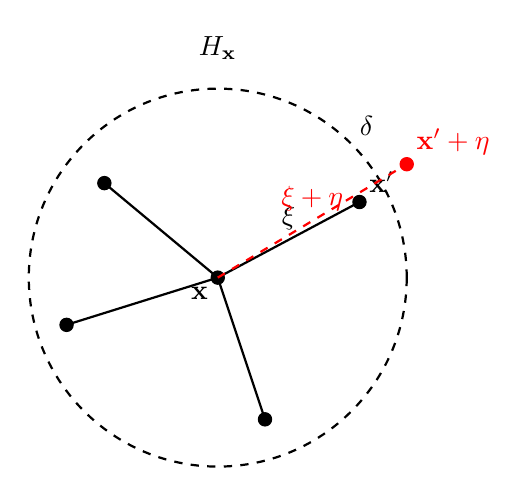
\begin{tikzpicture}[scale=1.2]
    % horizon
    \draw[dashed, thick] (0,0) circle (2);
    \node[above right] at (1.4,1.4) {$\delta$};
    % 中心点
    \filldraw (0,0) circle (2pt) node[below left] {$\mathbf{x}$};
    % 邻点与键
    \filldraw (1.5,0.8) circle (2pt) node[above right] {$\mathbf{x}'$};
    \draw[thick] (0,0) -- (1.5,0.8);
    \filldraw (-1.2,1.0) circle (2pt);
    \draw[thick] (0,0) -- (-1.2,1.0);
    \filldraw (0.5,-1.5) circle (2pt);
    \draw[thick] (0,0) -- (0.5,-1.5);
    \filldraw (-1.6,-0.5) circle (2pt);
    \draw[thick] (0,0) -- (-1.6,-0.5);
    % 标注 ξ 和 ξ+η
    \node[above] at (0.75,0.4) {$\boldsymbol{\xi}$};
    % 变形后位置
    \draw[dashed, thick, red] (0,0) -- (2.0,1.2);
    \filldraw[red] (2.0,1.2) circle (2pt);
    \node[red, above right] at (2.0,1.2) {$\mathbf{x}'+\boldsymbol{\eta}$};
    \node[red, above] at (1.0,0.6) {$\boldsymbol{\xi}+\boldsymbol{\eta}$};
    % horizon标签
    \node[above] at (0,2.2) {$H_{\mathbf{x}}$};
  \end{tikzpicture}
  \caption{近场范围与键的示意图，材料点 $\mathbf{x}$ 与其 horizon $H_{\mathbf{x}}$ 内所有点通过键相互作用}
  \label{fig:horizon-bond}
\end{figure}

图\ref{fig:horizon-bond}展示了近场范围与键的基本几何关系。近场范围 $\delta$ 的物理含义是材料点间相互作用的特征距离。当 $\delta$ 趋于零时，相互作用退化为无穷小邻域内的局部作用，近场动力学方程在形式上回到经典理论 \cite{SillingLehoucq2008}，因此经典连续介质力学可以看作近场动力学在零近场范围极限下的特例。$\delta$ 也常与材料的微结构尺度相联系：对于多晶金属可取为晶粒尺寸的量级，对于混凝土可取为骨料尺寸的量级。实际应用中 $\delta$ 的选取还需兼顾数值收敛性，通常要求近场域内包含足够多的物质点 \cite{Bobaru2009,BobaruHu2012}。

键（bond）是近场动力学的基本相互作用单元。连接 $\mathbf{x}$ 与 $\mathbf{x}'$ 的键在参考构型中的方向矢量记为 $\boldsymbol{\xi}=\mathbf{x}'-\mathbf{x}$，变形后的相对位移记为 $\boldsymbol{\eta}=\mathbf{u}(\mathbf{x}',t)-\mathbf{u}(\mathbf{x},t)$，键的伸长（stretch）定义为
\[
  s=\frac{|\boldsymbol{\xi}+\boldsymbol{\eta}|-|\boldsymbol{\xi}|}{|\boldsymbol{\xi}|}
\]
本构关系通过对力函数 $\mathbf{f}$ 描述。对线弹性微弹性材料，在小变形下对力函数可线性化为
\[
  \mathbf{f}(\boldsymbol{\eta},\boldsymbol{\xi})\approx \mathbf{C}(\boldsymbol{\xi})\,\boldsymbol{\eta}
\]
其中 $\mathbf{C}(\boldsymbol{\xi})$ 称为微观模量（micromodulus）函数，它描述了键的刚度随键长与方向的分布，其具体形式可通过令近场动力学的应变能密度在均匀变形下与经典应变能密度一致来确定 \cite{Silling2000,Silling2010}。

近场动力学与经典理论的关系值得进一步说明。一方面，线性化后的近场动力学在大尺度行为上与经典线弹性理论一致 \cite{Silling2000,Silling2010}，这是它可以作为经典理论推广的根本原因。另一方面，两者在小尺度行为上存在差异，近场动力学具有固有的非线性色散特性，波速依赖波数，这一差异在冲击与高频波问题中不可忽略 \cite{SillingLehoucq2010}。此外，给定一个经典材料，可以构造出多个近场动力学材料在均匀变形下与其等价，即一个经典材料对应多个近场动力学材料，因此从经典参数到微观模量的映射并不唯一，需要额外的约定。

近场动力学最突出的能力是裂纹的自发萌生与扩展（autonomous crack propagation）。裂纹在近场动力学中不是被预先定义的对象，而是键断裂的自然结果：当某个键的伸长超过临界值时，该键永久失效，众多键的失效累积便构成裂纹面。这一机制使裂纹的萌生 \cite{SillingWeckner2010}、扩展与分叉 \cite{HaBobaru2010} 以及多裂纹的相互作用都可以在同一套方程下自动产生，无需任何外部断裂准则。裂纹的萌生、扩展与路径选择全部内生于运动方程与本构模型，这正是近场动力学与经典断裂力学在方法论上的根本分别。图\ref{fig:bond-breakage}示意了键网络从完整到逐步断裂并最终形成裂纹面的过程：断裂并非一次性地插入裂纹，而是大量键在不同时刻独立失效的渐进累积——这一“自下而上”的断裂机制使得裂纹的萌生、扩展与分叉都成为解的组成部分，无需任何外部准则介入。

\begin{figure}[htbp]
  \centering
  \begin{tikzpicture}[scale=0.7]
    % (a) 完整键网络
    \begin{scope}
      \foreach \x in {0,1,2,3} {
          \foreach \y in {0,1,2} {
              \filldraw (\x,\y) circle (3pt);
            }
        }
      \foreach \x in {0,1,2} {
          \foreach \y in {0,1,2} {
              \draw[thin] (\x,\y) -- (\x+1,\y);
              \draw[thin] (\x,\y) -- (\x,\y+1);
              \draw[thin] (\x,\y) -- (\x+1,\y+1);
            }
        }
      \node[below] at (1.5,-0.5) {(a) 完整键网络};
    \end{scope}
    % (b) 部分键断裂
    \begin{scope}[xshift=5cm]
      \foreach \x in {0,1,2,3} {
          \foreach \y in {0,1,2} {
              \filldraw (\x,\y) circle (3pt);
            }
        }
      \foreach \x in {0,1,2} {
          \foreach \y in {0,1,2} {
              \draw[thin] (\x,\y) -- (\x+1,\y);
              \draw[thin] (\x,\y) -- (\x,\y+1);
              \draw[thin] (\x,\y) -- (\x+1,\y+1);
            }
        }
      % 断裂的键
      \draw[red, ultra thick] (1,1) -- (2,1);
      \node[red] at (1.5,1.3) {$\times$};
      \draw[red, ultra thick] (0,1) -- (1,1);
      \node[red] at (0.5,1.3) {$\times$};
      \draw[red, ultra thick] (1,0) -- (2,1);
      \node[red] at (1.3,0.3) {$\times$};
      \node[below] at (1.5,-0.5) {(b) 键逐步断裂};
    \end{scope}
    % (c) 裂纹面形成
    \begin{scope}[xshift=10cm]
      \foreach \x in {0,1,2,3} {
          \foreach \y in {0,1,2} {
              \filldraw (\x,\y) circle (3pt);
            }
        }
      \foreach \x in {0,1,2} {
          \foreach \y in {0,1,2} {
              \draw[thin] (\x,\y) -- (\x+1,\y);
              \draw[thin] (\x,\y) -- (\x,\y+1);
              \draw[thin] (\x,\y) -- (\x+1,\y+1);
            }
        }
      % 裂纹面
      \draw[red, ultra thick] (0,1) -- (3,1);
      \node[below] at (1.5,-0.5) {(c) 裂纹面形成};
    \end{scope}
  \end{tikzpicture}
  \caption{键断裂与裂纹形成过程，裂纹是键失效的自然累积结果，无需预设裂纹路径}
  \label{fig:bond-breakage}
\end{figure}

将近场动力学与分子动力学（MD）类比是有益的。两者都通过求和（积分）计算粒子（材料点）所受的力，运动方程的形式相近。但近场动力学是连续介质理论，不需要知道原子间势；其材料具有参考构型的记忆，本构关系基于变形而非势能面，因此可以描述具有复杂本构行为的工程材料，并可与经典连续介质力学的本构模型直接对接 \cite{Silling2000,Seleson2009}。

综上，近场动力学具有五个基本特征：
\begin{enumerate}
  \item \textbf{非局部性}。材料点与近场范围内所有点相互作用，作用范围由 $\delta$ 刻画，经典局部作用是其极限情形。
  \item \textbf{积分方程替代偏微分方程}。运动方程不含空间导数，这是其能够处理不连续的根本原因。
  \item \textbf{不连续性的自然处理}。裂纹等强不连续不需要特殊数学处理即可进入方程。
  \item \textbf{自主断裂模拟能力}。裂纹的萌生、分叉与汇合由方程自发产生，无需外部断裂准则。
  \item \textbf{多尺度桥梁潜力}。同一套方程适用于从原子尺度到连续介质尺度的描述，为跨尺度耦合提供了统一框架 \cite{Seleson2009,Silling2011coarsening}。
\end{enumerate}

\section{近场动力学的发展历程与研究现状}

自 2000 年创始论文发表以来，近场动力学经历了从单一键基模型到完整理论体系、从二维小规模算例到三维大规模工程应用的快速发展。本节按研究方向系统梳理其发展脉络，图\ref{fig:pd-timeline}给出了2000年以来的关键发展里程碑。从时间线上可清晰地识别三个关键跳跃：2000年键基理论奠定基础，2007年态基理论突破泊松比限制，2012年后开源软件（Peridigm）与手册的问世标志着近场动力学从学术研究走向工程应用的转型。本节后续各小节将沿上述线索逐一展开。

\begin{figure}[htbp]
  \centering
  \begin{tikzpicture}[scale=1.0]
    % 时间轴
    \draw[thick, -Stealth] (0,0) -- (13.0,0) node[right] {年份};
    % 里程碑（上方标签与下方标签交替排列，避免文字拥挤）
    \foreach \x/\yr/\lab in {0.7/2000/PMB模型, 3.6/2007/态基理论, 6.5/2010/综述与线性化, 9.4/2014/疲劳模型, 12.2/2020+/大规模应用} {
        \draw[thick] (\x,0) -- (\x,0.3);
        \node[above, font=\small] at (\x,0.3) {\yr};
        \node[font=\small, text width=3.5cm, align=center] at (\x,0.95) {\lab};
      }
    \foreach \x/\yr/\lab in {2.2/2005/EMU方法, 5.0/2008/LAMMPS-PD, 7.9/2012/Peridigm, 10.8/2016/PDDO与手册} {
        \draw[thick] (\x,0) -- (\x,0.3);
        \node[above, font=\small] at (\x,0.3) {\yr};
        \node[font=\small, text width=3.5cm, align=center] at (\x,-0.55) {\lab};
      }
  \end{tikzpicture}
  \caption{近场动力学发展里程碑（2000年至今）}
  \label{fig:pd-timeline}
\end{figure}

\subsection{本构理论的发展}

本构理论是近场动力学发展的主线之一。键基理论方面，Gerstle、Sau 与 Silling 将键基模型推广到混凝土结构分析 \cite{Gerstle2007}；Zhu 与 Ni 在键基理论中引入键的转动效应，使键基模型得以描述更一般的泊松比 \cite{ZhuNi2017}。态基理论方面，Silling 等建立了态基（state-based）框架 \cite{Silling2007}，以向量值态映射替代键基理论中仅依赖于单键变形的标量力函数，从根本上解除了键基模型泊松比固定为 1/4 的限制；Warren 等给出了非常规态基理论的数值实现并用于变形与断裂分析 \cite{Warren2009}，Silling 随后建立了态基理论的线性化体系 \cite{Silling2010}。本构对应（constitutive correspondence）原理是连接近场动力学与经典本构的桥梁：Silling 等在态基理论中首次提出对应机制 \cite{Silling2007}，Tupek、Rimoli 与 Radovitzky 将经典连续损伤模型嵌入态基近场动力学 \cite{TupekRimoli2013}，Tupek 与 Radovitzky 进一步将对应框架推广到非线性键应变度量 \cite{TupekRadovitzky2014}；Foster、Silling 与 Chen 发展了近场动力学粘塑性模型 \cite{Foster2010}。近期，Javili 等从连续运动学出发构造了新型近场动力学形式 \cite{Javili2019}，为非局部本构设计提供了新的思路。

图\ref{fig:pd-tree}给出了近场动力学本构模型的整体分类：从键基理论（BB-PD）出发，以单键轴向变形描述相互作用；常规态基理论（OSB-PD）将力密度与键的伸长方向解耦，解除了泊松比限制；非常规态基理论（NOSB-PD）通过变形梯度构造近似经典应力张量，实现经典本构向近场动力学框架的直接映射。
\begin{figure}[htbp]
  \centering
  
\includegraphics[width=0.9\textwidth]{diehl2022_fig2.png}
  \caption{近场动力学模型的分类示意（图片来源\cite{Diehl2022}）}
  \label{fig:pd-tree}
\end{figure}

图\ref{fig:pd-models}从相互作用方式角度直观对比了三者的核心差异：键基模型仅传递沿键方向的轴向力，常规态基在保持沿键方向传力的同时解除了力对键方向的依赖，非常规态基则允许键上存在任意方向的力以等价于经典连续介质力学中的一般应力状态。

\begin{figure}[htbp]
  \centering
  
\includegraphics[width=0.9\textwidth]{diehl2022_fig3.png}
  \caption{键基、常规态基与非常规态基三类本构模型的对比（图片来源\cite{Diehl2022}）}
  \label{fig:pd-models}
\end{figure}

本构理论的新进展主要体现在三个方向。其一，各向异性材料本构得到系统发展，Scabbia、Zaccariotto 与 Galvanetto 提出了适用于一般各向异性材料的常规态基近场动力学格式 \cite{Scabbia2024}，将各向异性弹性与断裂纳入统一的态基框架。其二，机器学习开始进入本构建模，Xu、D'Elia 与 Foster 建立了带物理约束的机器学习近场动力学本构框架 \cite{Xu2021}，通过学习微观模量等本构信息，为非局部本构的标定提供了数据驱动的新途径。其三，对应格式的稳定性问题受到持续关注，Silling 从势能最小化出发导出了态基材料的稳定性条件，指出对应材料模型可能因零能模式而失稳，并给出了修正应变能密度以消除零能模式的方案 \cite{Silling2017}。

\subsection{数值离散方法与边界条件}

数值方法是近场动力学走向应用的必经之路。Silling 与 Askari 的 EMU 方法采用均匀网格与中点求积 \cite{SillingAskari2005}，将运动方程对每个离散节点逐个求和计算内力并以显式时间积分推进，至今仍是应用最广泛的离散方案。围绕该方案，收敛性与自适应问题得到系统研究：Bobaru 等在一维问题中建立了收敛、自适应细化与尺度关系 \cite{Bobaru2009}，Seleson 与 Littlewood 对网格无关近场动力学模拟的收敛性进行了系统的数值研究 \cite{SelesonLittlewood2016}；Littlewood 在 Peridigm 中实现了动态断裂的自适应细化与接触模拟 \cite{Littlewood2010}。非常规态基理论中基于变形梯度近似的离散存在零能模式（zero-energy mode）问题，Wu 与 Ren 提出了稳定化方案 \cite{WuRen2015}。此外，配点型（collocation）离散的精度与稳定性分析也日益完善 \cite{SelesonLittlewood2016}。与离散格式紧密关联的另一类问题是边界条件的处理与表面效应。

近场动力学的边界条件具有特殊性：经典理论中的面力边界条件在近场动力学中必须转化为体积力形式施加于边界附近的薄层区域 \cite{SillingLehoucq2010}。由于近表面材料点的近场域不完整，其有效刚度与内部存在差异，这一现象称为表面效应（surface effect）或皮肤效应（skin effect）。Le 与 Bobaru 系统比较了多种表面修正方法在弹性与断裂问题中的效果 \cite{LeBobaru2018}；Mitchell、Silling 与 Littlewood 提出位置感知（position-aware）本构，从本构层面减轻表面效应 \cite{Mitchell2015}。近场范围与边界的相互作用还催生了变近场域（variable horizon）方法，Ren、Zhuang 与 Rabczuk 提出的双近场域（dual-horizon）近场动力学保证了变近场域离散下的力平衡 \cite{Ren2017dualhorizon}。

离散格式的收敛性分析还揭示出近场动力学与经典无网格方法之间的深层联系，图\ref{fig:pd-convergence}给出了收敛性概念示意。近场动力学的数值收敛需区分两种机制，二者与离散网格步长 $\Delta x$ 和近场范围 $\delta$ 的比值 $m=\delta/\Delta x$（即近场域内沿某一方向包含的物质点数目）密切相关。其一是 $\delta$ 收敛（$\delta$-convergence）：固定比值 $m$，逐步缩小近场范围 $\delta$，使材料点间的相互作用距离不断缩短、非局部效应逐渐消失，此时近场动力学解收敛于经典局部理论解。$\delta$ 收敛检验的是模型层面：非局部模型在何种条件下退化为局部模型，是近场动力学与经典连续介质力学相容性的数值体现。其二是 $m$ 收敛（$m$-convergence）：固定近场范围 $\delta$，仅细化离散网格、增大 $m$，使近场域内的物质点数目不断增多，积分求积误差随之减小，此时近场动力学解收敛于该 $\delta$ 取值下非局部模型的精确解。$m$ 收敛检验的是数值层面：在非局部模型固定不变的前提下，离散格式逼近该模型真解的程度。正确区分二者是评估近场动力学数值精度的前提：$\delta$ 收敛验证模型本身，$m$ 收敛验证数值格式。Ganzenm\"uller、Hiermaier 与 May 指出，采用节点积分的近场动力学离散与光滑粒子流体动力学在数学上等价，因而同样面临零能模式等无网格方法的固有困难 \cite{Ganzenmuller2015}；Bessa、Foster、Belytschko 与 Liu 将再生核粒子方法与近场动力学统一，提出了再生核近场动力学（reproducing kernel peridynamics），为正则化与稳定性分析提供了新工具 \cite{Bessa2014}；Dipasquale、Zaccariotto 与 Galvanetto 则发展了二维近场动力学的自适应网格细化格式，在裂纹前沿动态加密离散，兼顾了精度与效率 \cite{Dipasquale2014}。

\begin{figure}[htbp]
  \centering
  
\includegraphics[width=0.57\textwidth]{diehl2022_fig5.png}
  \caption{近场动力学数值方法的收敛性示意（图片来源\cite{Diehl2022}）}
  \label{fig:pd-convergence}
\end{figure}

\subsection{断裂与损伤}

断裂模拟是近场动力学最具代表性的应用领域。动态断裂方面，Ha 与 Bobaru 系统研究了动态裂纹扩展与分叉 \cite{HaBobaru2010}，发现近场范围相对于材料特征尺度的选取对分叉角度和分叉数量有决定性作用，为近场动力学在高速冲击断裂中的应用提供了参数选取依据。Bobaru 与 Hu 进一步研究了近场范围的选择对裂纹分叉模式的影响 \cite{BobaruHu2012}；Agwai 等将近场动力学结果与实验对比，验证了其在裂纹扩展预测中的可靠性 \cite{Agwai2011}；Zhou、Wang 与 Qian 用扩展非常规态基近场动力学模拟了脆性材料的裂纹偏转与分叉 \cite{ZhouWang2016}。疲劳方面，Silling 与 Askari 提出近场动力学疲劳模型，键的剩余寿命随循环载荷下的伸长循环而消耗，从而在单一模型内同时模拟疲劳裂纹的萌生、扩展与最终失效 \cite{SillingAskari2014}。损伤与断裂的过渡是近场动力学的独特优势：连续损伤通过键的渐进失效自然演化为离散裂纹 \cite{TupekRimoli2013}，多裂纹的萌生、汇合与相互作用也无需额外的拓扑处理 \cite{WangZhou2016}。

断裂模拟的可靠性需要通过基准实验加以验证。Diehl 等系统综述了可用于近场动力学模型验证的基准实验 \cite{Diehl2019}，并进一步将近场动力学与相场断裂模型在若干工程基准算例上进行了定量对比 \cite{Diehl2022}，图\ref{fig:pd-sandia}给出了其中断裂挑战赛算例的实验设置示意：该挑战赛要求参赛者仅凭初始几何与材料参数预测裂纹路径，近场动力学凭借其无需预设裂纹路径的自主断裂能力，在定量预测精度上表现出色，充分验证了该方法的工程适用性。此类对比研究为近场动力学模型的适用范围与参数标定提供了依据：在裂纹萌生与动态扩展问题上，近场动力学无需预设裂纹路径即可自动捕捉断裂过程；而相场模型则通过扩散界面近似描述损伤带，二者的互补性已成为当前断裂模拟研究的热点。

\begin{figure}[htbp]
  \centering
  
\includegraphics[width=0.42\textwidth]{diehl2022_fig7.png}
  \caption{Sandia 断裂挑战赛基准算例的实验设置示意（图片来源\cite{Diehl2022}）}
  \label{fig:pd-sandia}
\end{figure}

\subsection{多尺度耦合}

近场动力学的计算成本远高于经典局部理论，因此将非局部区域限制在裂纹可能出现之处、其余区域采用经典理论，是兼顾精度与效率的自然选择。Macek 与 Silling 最早展示了在有限元框架内实现近场动力学的方法 \cite{Macek2007}；Zaccariotto 等将有限元网格与近场动力学网格耦合 \cite{Zaccariotto2018}；Lubineau 等提出 morphing 方法，引入反映局部-非局部权重连续变化的过渡区（morphing zone），使材料能量泛函平滑切换，避免了直接耦合在界面处的不平衡力 \cite{Lubineau2012}；Han 等将该方法推广到态基近场动力学 \cite{Han2016morphing}；Wang、Kulkarni 与 Tabarraei 提出了近场动力学与经典弹性的并发耦合方法 \cite{Wang2019coupling}；Sun 与 Fish 发展了基于叠加的耦合格式 \cite{SunFish2019}。

上述耦合格式可按理论构造分为力型、能量型与叠加型三类：力型耦合在界面或重叠区直接建立力平衡；能量型耦合通过过渡区的能量泛函实现局部与非局部理论的统一变分表述；叠加型耦合则将经典弹性解与近场动力学修正解叠加。三类框架在稳定性、精度与实现成本上各有取舍，其构造细节与误差分析将在第 12 章展开。在原子与连续介质之间，Silling 提出了用于分子动力学与近场动力学的粗化方法 \cite{Silling2011coarsening}，从原子位移场推导出一套计算粗粒化近场动力学力的系统程序，使近场动力学本构可直接从分子动力学模拟中提取；Seleson 等则论证了近场动力学可以作为分子动力学的尺度提升（upscaling）框架 \cite{Seleson2009}，为跨越多个尺度的统一建模提供了可能。

\subsection{多物理场与近场动力学微分算子}

近场动力学的非局部框架同样适用于多物理场问题。Bobaru 与 Duangpanya 建立了含演化不连续体的瞬态热传导近场动力学格式 \cite{BobaruDuangpanya2010}，将温度梯度替换为温度差的积分形式，使热传导方程在含裂纹的含时演化问题中同样有效；Oterkus、Madenci 与 Agwai 建立了全耦合的近场动力学热力学理论，并模拟了热冲击下的断裂 \cite{Oterkus2014}。在扩散与化学腐蚀方面，Chen 与 Bobaru 建立了点蚀腐蚀损伤的近场动力学模型，将溶解过程与力学损伤统一在同一框架内 \cite{ChenBobaru2015}：腐蚀引起的材料溶解通过键的逐步失效表征，力学载荷加速损伤演化，溶解则持续削弱键的承载能力，二者形成正反馈直至最终失效。热力耦合、扩散力学耦合与腐蚀疲劳等问题的近场动力学建模已成为当前研究热点之一 \cite{Bobaru2016}。在统一的非局部框架下，近场动力学微分算子（PDDO）将上述思想进一步推广。

Madenci、Barut 与 Futch 提出的近场动力学微分算子（peridynamic differential operator，简称 PDDO）以积分形式构造任意阶导数 \cite{Madenci2016}，使经典偏微分方程可以在非局部框架内求解，并在拓扑优化、图像处理、结构分析等领域得到应用。基于近场动力学的损伤感知优化设计也吸引了越来越多研究者的关注，近场动力学在其中扮演着结构响应与损伤演化预测器的角色 \cite{Madenci2016,MadenciOterkus2014}。

多物理场近场动力学在工程问题中的应用日益广泛。在水力压裂方面，Ouchi 等建立了孔隙流动与地质力学完全耦合的近场动力学模型，实现了流体驱动裂纹扩展的模拟，并验证了与经典解的一致性 \cite{Ouchi2015}；顾鑫、章青与 Madenci 对多物理场耦合分析的近场动力学理论与方法进行了系统总结 \cite{GuZhang2019}。在结构优化方面，基于近场动力学的拓扑优化方法快速发展，Vieira 与 Ara\'ujo 提出了改进的密度法拓扑优化框架，实现了网格无关的优化结果，并可直接处理含裂纹结构的拓扑优化问题 \cite{Vieira2024}。PDDO 的应用领域也持续拓展，Madenci 等将其推广到数据估计、图像压缩与恢复以及模型降阶等非传统领域 \cite{Madenci2022}。

\subsection{国内研究进展}

在软件工具方面，Sandia 国家实验室的开源代码 Peridigm \cite{Peridigm2012}、LAMMPS 中的近场动力学模块 \cite{Parks2008} 以及商业软件 LS-DYNA 中的实现 \cite{WuRen2015} 为近场动力学的工程应用提供了基础平台，Diehl 等的基准实验综述 \cite{Diehl2019} 则为模型验证提供了依据。国内近年在近场动力学开源代码方面也有长足发展，相关内容将在第17章和第18章详述。

近场动力学在中国得到了快速发展。重庆大学周小平团队在扩展非常规态基近场动力学与岩石断裂模拟方面成果突出，模拟了脆性材料在动态载荷下的裂纹偏转与分叉 \cite{ZhouWang2016}，以及岩体压剪载荷下缺陷的扩展与汇合 \cite{WangZhou2016}；河海大学朱其志团队在键基理论中引入键的转动效应，拓展了键基模型的适用范围 \cite{ZhuNi2017}；任辉龙、庄晓莹与 Rabczuk 提出的双近场域近场动力学解决了变近场域离散的稳定性问题 \cite{Ren2017dualhorizon}。此外，大连理工大学、清华大学、北京航空航天大学、上海交通大学等高校的研究团队也在近场动力学理论、数值方法、多场耦合与工程应用方面开展了大量工作。国内学者的相关成果贯穿本书各章，在此不逐一列举。

国内学术界对近场动力学的发展也进行了系统的总结与展望。张恒、张雄与乔丕忠从断裂力学视角综述了近场动力学的理论框架、数值方法与典型应用，梳理了近场动力学在国内外的发展脉络与研究热点 \cite{ZhangHeng2022}。这些综述工作与本书的章节安排相互印证：近场动力学已从理论方法研究走向工程应用，国内学者在岩石断裂、多物理场耦合、算法开发与软件实现等方面正逐步形成具有特色的研究体系。

\section{本书的结构与使用指南}

本书共 19 章和 5 个附录，按逻辑组织为六个部分。

第一部分为理论基础，包括第 1 至 3 章。第 1 章（本章）回答为什么需要近场动力学以及它是什么；第 2 章建立近场动力学的基本理论框架，包括物质点、键、近场域与族等基本概念，变形与受力的描述，守恒律以及损伤与断键准则；第 3 章严格分析近场动力学与经典连续介质力学的关系，包括局部极限、近场动力学应力张量、渐近相容性与非局部变分原理。

第二部分为本构理论，包括第 4 至 8 章，依次介绍键基理论（第 4 章）、键基理论的改进（第 5 章）、常规态基理论（第 6 章）、非常规态基理论（第 7 章）与本构建模的一般方法（第 8 章）。

第三部分为数值方法与断裂模拟，包括第 9 至 11 章，涵盖空间离散与时间积分（第 9 章）、边界条件的处理（第 10 章）以及裂纹与损伤的数值模拟（第 11 章）。

第四部分为耦合与多物理场，包括第 12 至 14 章：第 12 章介绍近场动力学与有限元的耦合，第 13 章介绍近场动力学热传导，第 14 章介绍热力、扩散与腐蚀等多物理场耦合问题。

第五部分为前沿与工具，包括第 15 至 18 章：第 15 章介绍近场动力学微分算子（PDDO）及其应用，第 16 章介绍近场动力学的前沿专题，第 17 章与第 18 章分别介绍程序设计基础与主流软件（Peridigm、LAMMPS 等）的使用。

第六部分为基准算例，即第 19 章，汇集了从简单拉伸到动态断裂的系列验证算例，便于读者检验自己的程序实现。

附录 A 给出数学补充，附录 B 回顾经典连续介质力学的基本内容，附录 C 给出部分程序代码，附录 D 为全书符号表，附录 E 为补充参考文献。全书整体结构可参见图\ref{fig:book-structure}：六个部分构成从理论到实践的完整递进链——理论基础（第1--3章）建立概念框架，本构理论（第4--8章）提供材料模型，数值方法与断裂模拟（第9--11章）实现求解，耦合与多物理场（第12--14章）拓展应用边界，前沿与工具（第15--18章）连接研究前沿与工程实践，基准算例（第19章）提供验证平台。

\begin{figure}[htbp]
  \centering
  \begin{tikzpicture}[
      box/.style={draw, thick, rounded corners, minimum width=3.5cm, minimum height=1.2cm, align=center, font=\small},
      arrow/.style={-Stealth, thick}
    ]
    \node[box, fill=blue!10] (p1) at (0,0) {第一部分\\理论基础\\第1--3章};
    \node[box, fill=green!10] (p2) at (4.5,0) {第二部分\\本构理论\\第4--8章};
    \node[box, fill=orange!10] (p3) at (9,0) {第三部分\\数值与断裂\\第9--11章};
    \node[box, fill=red!10] (p4) at (0,-2) {第四部分\\耦合与多物理场\\第12--14章};
    \node[box, fill=purple!10] (p5) at (4.5,-2) {第五部分\\前沿与工具\\第15--18章};
    \node[box, fill=gray!10] (p6) at (9,-2) {第六部分\\基准算例\\第19章};
    \draw[arrow] (p1) -- (p2);
    \draw[arrow] (p2) -- (p3);
    \draw[arrow] (p3) -- (p4);
    \draw[arrow] (p4) -- (p5);
    \draw[arrow] (p5) -- (p6);
  \end{tikzpicture}
  \caption{本书结构概览，六部分构成从理论到实践的完整体系}
  \label{fig:book-structure}
\end{figure}

针对不同的读者，本书推荐如下阅读路径。以近场动力学为研究方向的研究生，可按顺序通读全书，重点研读第 2、3 章的理论推导与第 4 至 8 章的本构理论，并配合第 19 章的算例动手实现。具有力学背景、希望尽快开展数值模拟的工程技术人员，可先读第 1 章和第 9 至 11 章，掌握离散方法与断裂模拟的基本流程，再根据需要查阅第 4 至 8 章的本构细节。对理论数学感兴趣的读者，可在第 1 至 3 章的基础上结合附录 A、B 深究近场动力学的数学基础。

阅读本书需要具备弹性力学、连续介质力学与有限元方法的基本知识，并对张量分析和变分法有初步了解。附录 B 对经典连续介质力学作了系统回顾，供读者随时查阅。全书采用统一的符号约定，主要符号见附录 D。

\begin{remark}
  本书各章之间的衔接关系可概括为：第 1 章提出问题并给出整体图景，第 2、3 章奠定理论，第 4 至 8 章丰富本构，第 9 至 11 章实现数值求解，第 12 至 16 章拓展应用边界，第 17 至 19 章落地为可运行的程序与算例。读者在阅读任一章节时，都可以在本书的结构中找到其位置与前后依赖关系。
\end{remark}
